\documentclass[a4paper, 12pt]{article}
\usepackage[utf8]{inputenc}
\usepackage[english,russian]{babel}
\usepackage[warn]{mathtext}
\usepackage{graphicx}
\usepackage{float}
\restylefloat{table}
\usepackage{amsmath}
\usepackage{floatflt}
\usepackage[T2A]{fontenc}
\usepackage[left=20mm, top=20mm, right=20mm, bottom=20mm, footskip=10mm]{geometry}

\tolerance 1414
\hbadness 1414
\emergencystretch 1.5em
\hfuzz 0.3pt        % размер максимального переполнения без warning'a
\widowpenalty=10000 % запрещает одиночную строку абзаца в начале страницы
\vfuzz \hfuzz
\raggedbottom       % если на странице мало содержимого, добавить пустое место в конце, а не в середине страницы



\begin{document}

\begin{titlepage}
	\centering
	\vspace{5cm}
	{\scshape\LARGE московский физико-технический институт (национальный исследовательский университет) \par}
	\vspace{6cm}
	{\scshape\Large Лабораторная работа 3.6.1 (150А) \par}
	{\huge\bfseries Спектральный анализ электрических сигналов\par}
	\vspace{1cm}
	\vfill
\begin{flushright}
	{\large Б03-102}\par
	\vspace{0.3cm}
	{\LARGE Куланов Александр}
\end{flushright}
	

	\vfill


	Долгопрудный, 2022 г.
\end{titlepage}

\begin{itemize}
	\item \textbf{Цель работы:} изучить спектры периодических электрических сигналов и сравнить их с рассчитанными теоретически
    \item \textbf{В работе используются:} компьютер, USB - осциллограф АКИП - 4107, функциональный генератор WaveStation 2012, соединительные кабели
    
\end{itemize}

\section{Экспериментальная установка}

\begin{figure}[h]
    \centering
    \includegraphics[width=0.85\textwidth]{set}
    \caption{Схема установки}
    \label{fig:set}
\end{figure}

Функциональный генератор WaveStation 2012 позволяет сформировать два различных электрических сигнала, 
которые выводятся на два независимых канала --- "CH1" и "CH2". Сигнал с канала "CH1" подается на вход "A", а 
сигнал с канала "CH2" --- на вход "B" USB-осциллографа. Затем эти сигналы подаются на вход компьютера через
USB-соединение. При работе USB-осциллографа в режиме осциллографа, на экране компьютера можно наблюдать каждый 
из сигналов в отдельности, а также их произведение. В режиме спектроанализатора можно наблюдать спектры этих сигналов.

При включении функционального генератора, на его экране отображается информация о параметрах электрического сигнала.
\begin{enumerate}
	\item Кнопка включения
	\item USB - разъём
	\item Экран
	\item Кнопки экранного меню
	\item Кнопки выбора типов сигналов
	\item Цифровая панель
	\item Функциональные кнопки
	\item Разъемы с кнопками включения (выключения) выходных сигналов
	\item Кнопки перемещения
	\item Подстроечный регулятор
\end{enumerate}

\begin{figure}[H]
    \centering
    \includegraphics[width=0.85\textwidth]{set1}
    \caption{Передняя панель функционального генератора}
    \label{fig:set1}
\end{figure}
 
\section{Теоретические сведения}
\subsection*{Разложение сложных сигналов на периодические колебания}

Пусть задана функция $f(t)$, которая периодически повторяется с частотой $\Omega_1 = \dfrac{2\pi}{T}$, где $T$ --- период повторения импульсов. Её разложение в ряд Фурье имеет вид 
\begin{equation}
f(t) = \dfrac{a_0}{2} + \sum\limits_{n = 1}^{\infty}\left[a_n \cos \left(n \Omega_1t\right) + b_n \sin \left(n \Omega_1t\right)\right]
\end{equation}
или
\begin{equation}
f(t) = \dfrac{a_0}{2} + \sum\limits_{n = 1}^{\infty}A_n \cos \left(n\Omega_1t-\psi_n\right).
\end{equation}
Если сигнал чётен относительно $t=0$, в тригонометрической записи остаются только члены с косинусами. Для нечетной наоборот.
Коэффициенты определяются по формуле
\begin{equation}
\begin{array}{c}
a_n  = \dfrac{2}{T}\int\limits_{t_1}^{t_1+T}f(t)\cos\left(n \Omega_1 t\right) dt,\\
\\
b_n = \dfrac{2}{T}\int\limits_{t_1}^{t_1+T}f(t)\sin\left(n \Omega_1 t\right) dt.
\end{array}
\end{equation}
Здесь $t_1$ --- время, с которого мы начинаем отсчет.
Сравнив формулы $(1)$ и $(2)$ можно получить выражения для $A_n$  и $\psi_n$:
\begin{equation}
\begin{array}{l}
A_n = \sqrt{a_n^2+b_n^2},\\
 \psi_n = \arctan \dfrac{b_n}{a_n}.
\end{array}
\end{equation}
\subsection*{Периодическая последовательность прямоугольных импульсов}
Введем величину: $\Omega_1 = \dfrac{2\pi}{T}$,
где $T$ --- период повторения импульсов.
Коэффициенты при косинусных составляющих будут равны
\begin{equation}
a_n = \dfrac{2}{T}\int\limits_{-\tau/2}^{\tau/2}V_0\cos\left(n\Omega_1 t\right)dt = 2V_0\dfrac{\tau}{T}\dfrac{\sin\left(n\Omega_1\tau/2\right)}{n\Omega_1\tau/2} \sim \dfrac{\sin x}{x}.
\end{equation}
Здесь $V_0$ - амплитуда сигнала.
Поскольку наша функция четная, то $b_n = 0$. 
Пусть $T$ кратно $\tau$. Тогда введем ширину спектра, равную $\Delta \omega$ --- расстояние от главного максимума до первого нуля огибающей, возникающего, как нетрудно убедиться при $n = \dfrac{2\pi}{\tau \Omega_1}$. При 
этом
\begin{equation}
\Delta \omega \tau \simeq 2\pi \Rightarrow \Delta \nu \Delta t \simeq 1.
\end{equation}

\begin{figure}[H]
    \centering
    \includegraphics[width=0.5\textwidth]{data/square.png}
    \caption{Прямоугольный сигнал}
    \label{fig:data/square.png}
\end{figure}
\begin{figure}[H]
    \centering
    \includegraphics[width=0.5\textwidth]{data/spsquare.png}
    \caption{Спектр прямоугольного сигнала}
    \label{fig:data/spsquare.png}
\end{figure}

\subsection*{Периодическая последовательность цугов}
Возьмём цуги колебания $V_0 \cos(\omega_0 t)$ с длительностью цуга $\tau$ и периодом повторений $T$.\\
Функция $f(t)$ снова является четной относительно $t = 0$. Коэффициент при $n$-ой гармонике согласно формуле $(3)$ равен
\begin{equation}
a_n = \dfrac{2}{T}\int\limits_{-\tau/2}^{\tau/2}V_0 \cos \left(\omega_0t\right) \cdot \cos\left(n \Omega_1t\right)dt = V_0 \dfrac{\tau}{T}\left( \dfrac{\sin\left[\left(\omega_0 - n \Omega_1\right)\dfrac{\tau}{2}\right]}{\left( \omega_0 - n \Omega_1\right) \dfrac{\tau}{2}} + \dfrac{\sin\left[\left(\omega_0 + n \Omega_1\right)\dfrac{\tau}{2}\right]}{\left( \omega_0 + n \Omega_1\right) \dfrac{\tau}{2}}\right).
\end{equation}
Пусть $T$ кратно $\tau$. Тогда спектры последовательности прямоугильных сигналов и цугов аналогичны, но максимумы сдвинуты на $\omega_0$.

\begin{figure}[H]
    \centering
    \includegraphics[width=0.5\textwidth]{data/zug.png}
    \caption{Цуги}
    \label{fig:data/zug.png}
\end{figure}
\begin{figure}[H]
    \centering
    \includegraphics[width=0.5\textwidth]{data/spzug.png}
    \caption{Спектр цугов}
    \label{fig:data/spzug.png}
\end{figure}
\subsection*{Амплитудно-модулированные колебания}
Рассмотрим гармонические колебания высокой частоты $\omega_0$, амплитуда которых медленно меняется по гармоническому закону с частотой $\Omega \ll \omega_0$.
\begin{equation}
f(t) = A_0 \left[1+m\cos \Omega t\right] \cos \omega_0 t.
\end{equation}
Коэффициент $m$ называется \textit{глубиной модуляции}. При $m < 1$ амплитуда меняется от минимальной $A_{min} = A_0(1-m)$ до максимальной $A_{max} = A_0(1+m)$. Глубина модуляции может быть представлена в виде
\begin{equation}
m = \dfrac{A_{max}-A_{min}}{A_{max}+A_{min}}.
\end{equation}
Простым тригонометрическим преобразованием уравнения $(8)$ можно найти спектр колебаний
\begin{equation}
f(t) = A_0 \cos \omega_0t + \dfrac{A_0m}{2} \cos \left(\omega_0 + \Omega\right)t + \dfrac{A_0m}{2}\cos\left(\omega_0 - \Omega\right)t.
\end{equation}

\begin{figure}[H]
    \centering
    \includegraphics[width=0.5\textwidth]{data/AM.png}
    \caption{Амплитудно-модулированный сигнал}
    \label{fig:data/AM.png}
\end{figure}
\begin{figure}[H]
    \centering
    \includegraphics[width=0.5\textwidth]{data/spAM.png}
    \caption{Спектр амплитудно-модулированного сигнала}
    \label{fig:data/spAM.png}
\end{figure}

\section{Обработка результатов}
\subsection{Прямоугольный сигнал}

Картины спектров прямоугольного сигнала для различных значений приведены на рисунках 10-15 приложения. 
При анализе картин стало ясно, что при возрастании $\tau$ в два раза, ширина спектра уменьшается в два раза и в два раза возрастает амплитуда.
Также $\Delta\nu$ сохраняется между гармониками.

\subsection{Цуги}

Картины спектров цугов для различных сигналов приведены на рисунках 16-19 приложения. При увеличении периода пульса в пять раза, амплитуда уменьшается в то
же количество раз. 

Построим график зависимости $\Delta \nu (1/\tau)$:
\begin{figure}[H]
    \centering
    \includegraphics[width=1\textwidth]{zugs_out.png}
    \caption{Зависимость $\Delta \nu (1/\tau)$}
    \label{fig:zugs_out.jpg}
\end{figure}
Как видно по графику, соотношение неопределенности хорошо выполняется.

\subsection{Амплитудная модуляция}

Выведем картину амплитудно-модулированного сигнала с глубиной модуляции 0.5, частотой 50 кГц и частотой модуляции 2 кГц (рисунок 20).
Проверим соотношение (9):
\begin{equation}
	m = \dfrac{A_{max}-A_{min}}{A_{max}+A_{min}} =  \dfrac{802}{1889} = 0.43
\end{equation}
Из формулы 10 следует, что $a_{\text{осн}} = A_0$, $a_{\text{бок}} = mA_0/2$.
Убедимся в этом, построив график (рисунок \ref{fig:am_out}). Как видно по графику, соотношение выполняется.
Угол наклона прямой равен \textbf{0.96}
\begin{figure}[H]
    \centering
    \includegraphics[width=1\textwidth]{am_out.png}
    \caption{К амплитудной модуляции}
    \label{fig:am_out}
\end{figure}

\section{Вывод}
Были исследованы несколько типов периодических сигналов и их разложение в гармонический спектр, получены картины спектров. Проверена справедливость нескольких соотношений, в том числе соотношения неопределенности.
\section{Приложение}
\subsection*{Прямоугольный сигнал}
\begin{figure}[H]
    \centering
    \includegraphics[width=0.7\textwidth]{data/1_30.jpg}
    \caption{$f = 1 kHz, \tau = 30 \mu s$}
    \label{fig:data/1_30.jpg}
\end{figure}
\begin{figure}[H]
    \centering
    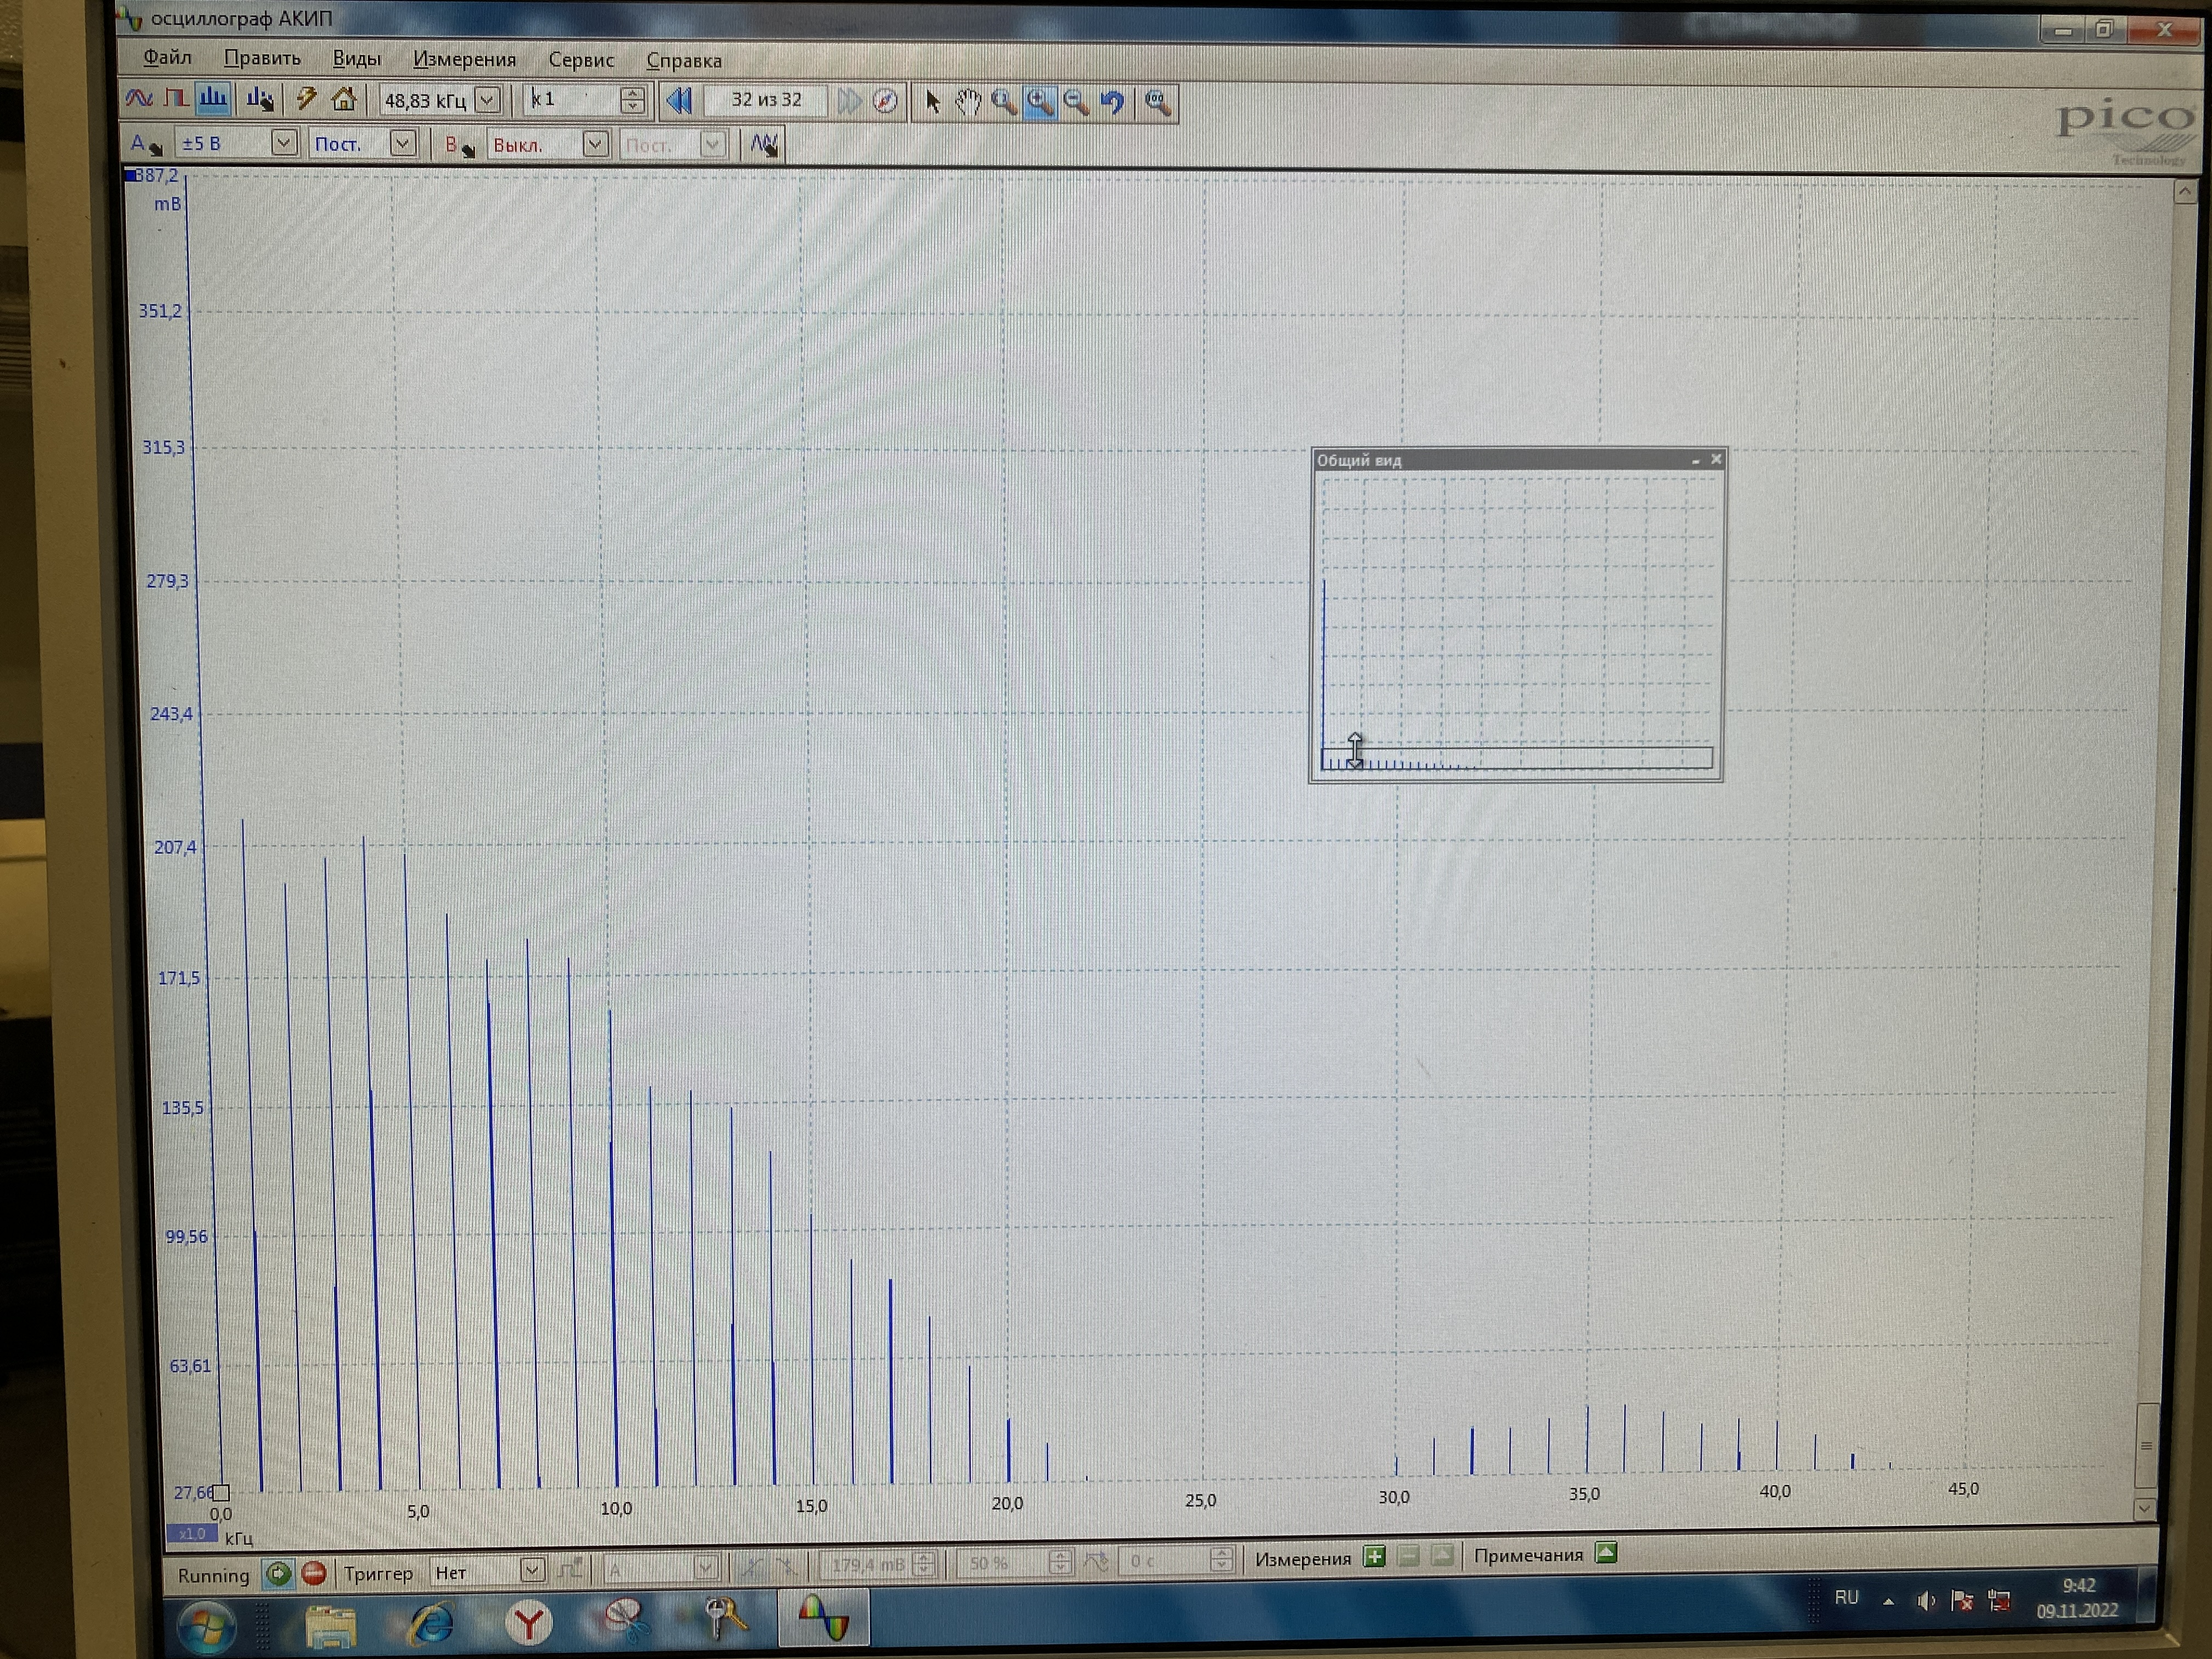
\includegraphics[width=0.7\textwidth]{data/1_40.jpg}
    \caption{$f = 1 kHz, \tau = 40 \mu s$}
    \label{fig:data/1_40.jpg}
\end{figure}
\begin{figure}[H]
    \centering
    \includegraphics[width=0.7\textwidth]{data/1_50.jpg}
    \caption{$f = 1 kHz, \tau = 50 \mu s$}
    \label{fig:data/1_50.jpg}
\end{figure}
\begin{figure}[H]
    \centering
    \includegraphics[width=0.7\textwidth]{data/2_20.jpg}
    \caption{$f = 2 kHz, \tau = 20 \mu s$}
    \label{fig:data/2_20.jpg}
\end{figure}
\begin{figure}[H]
    \centering
    \includegraphics[width=0.7\textwidth]{data/3_20.jpg}
    \caption{$f = 3 kHz, \tau = 20 \mu s$}
    \label{fig:data/3_20.jpg}
\end{figure}
\subsection*{Цуги}
\begin{figure}[H]
    \centering
    \includegraphics[width=0.7\textwidth]{data_zugs/1.jpg}
    \caption{$f = 50 kHz, \tau = 1 ms, N = 5$}
    \label{fig:data_zugs/1.jpg}
\end{figure}
\begin{figure}[H]
    \centering
    \includegraphics[width=0.7\textwidth]{data_zugs/2.jpg}
    \caption{$f = 50 kHz, \tau = 5 ms, N = 5$}
    \label{fig:data_zugs/2.jpg}
\end{figure}
\begin{figure}[H]
    \centering
    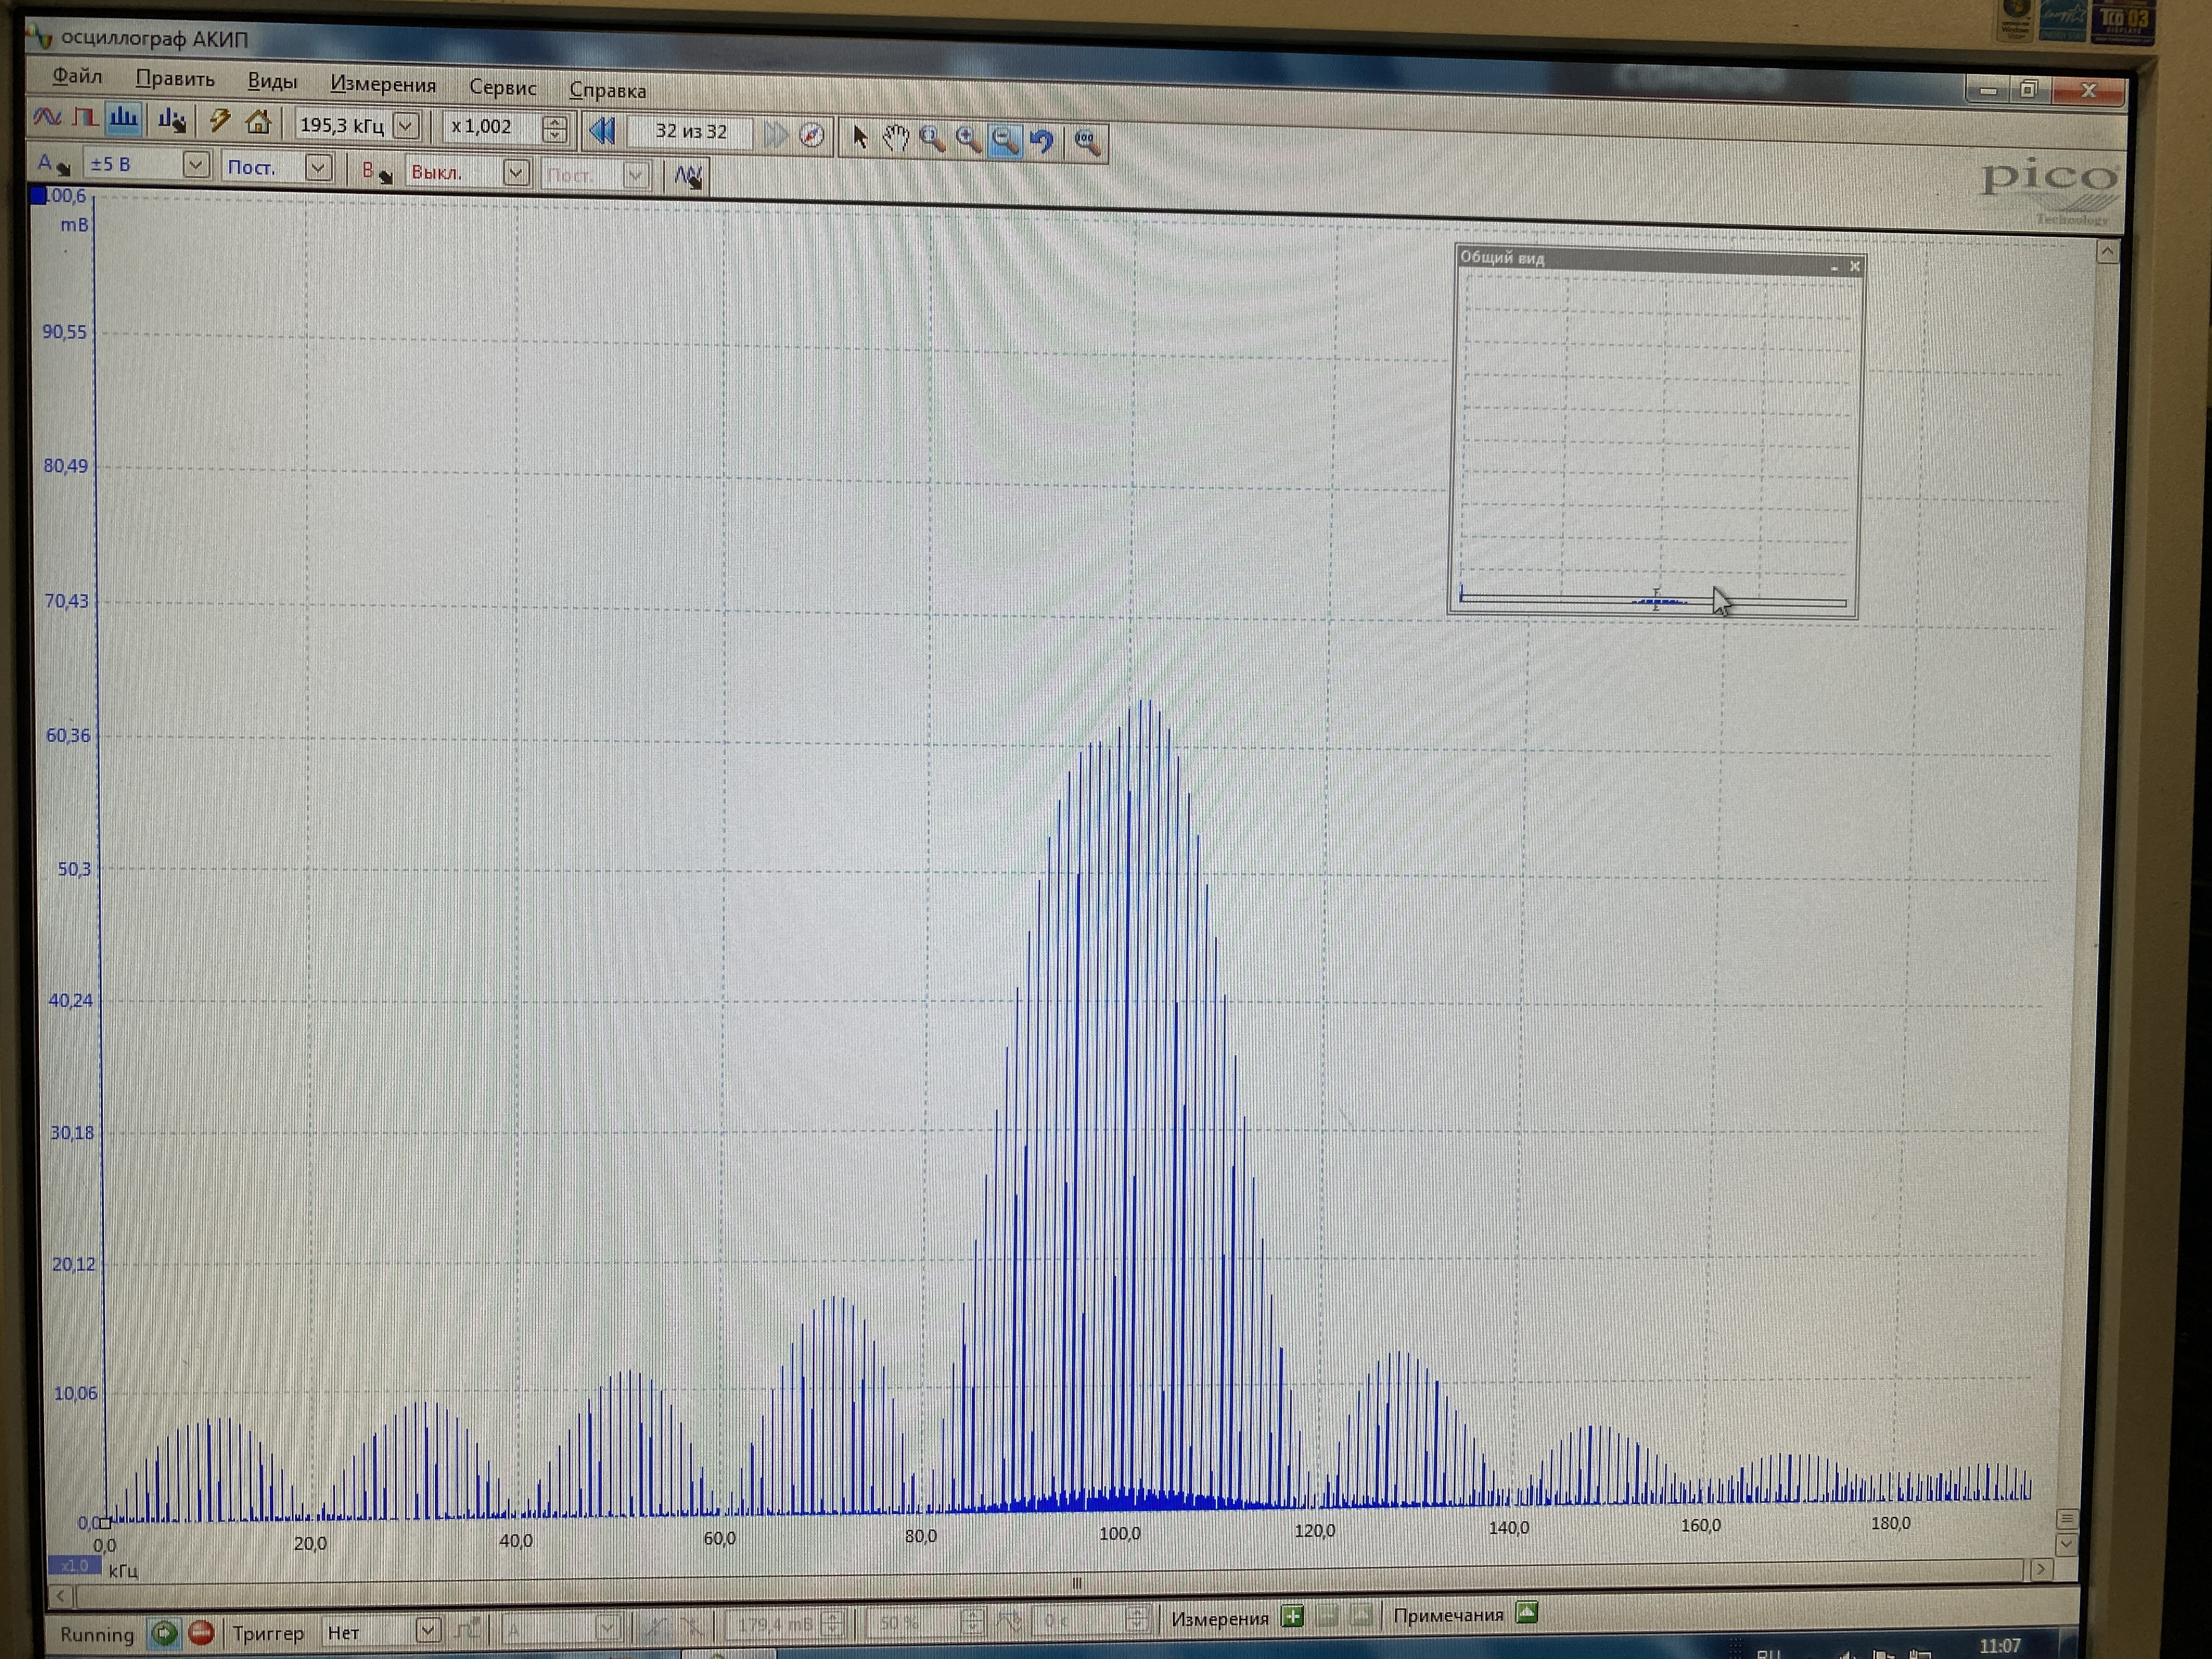
\includegraphics[width=0.7\textwidth]{data_zugs/3.jpg}
    \caption{$f = 100 kHz, \tau = 1 ms, N = 5$}
    \label{fig:data_zugs/3.jpg}
\end{figure}
\begin{figure}[H]
    \centering
    \includegraphics[width=0.7\textwidth]{data_zugs/4.jpg}
    \caption{$f = 50 kHz, \tau = 1 ms, N = 3$}
    \label{fig:data_zugs/4.jpg}
\end{figure}
\subsection*{Амплитудная модуляция}
\begin{figure}[H]
    \centering
    \includegraphics[width=0.7\textwidth]{data_am/1.jpg}
    \caption{Амплитудно-модулированный сигнал, глубина 0.5}
    \label{fig:data_am/1.jpg}
\end{figure}


\end{document}